The next question is designed to ask the participants which networking library they use. Although the network library's use does not directly affect maintainability, this question was included in the questionnaire. It was also among the aims of this study to identify developer tendencies. Also, the use of some advanced networking libraries indirectly affects maintainability due to the out of box solutions they offer. For this reason, it was deemed appropriate to add this question to the survey. When looking at the answers, it is seen that the Retrofit / OkHttp library is dominating. It is observed that 75.6\% of the participants use only this library and approximately 13.8\% prefer Retrofit/OkHttp libraries and other libraries. The graphical breakdown of responses is presented below in Fig. \ref{fig:networking_lib}. It would not be wrong to say that this library is mainly preferred due to its ease when integrating back-end systems running on REST architecture into Android applications. Besides, it is seen that 9.4\% (the second-highest rate) of the participants stated that they also used the Apollo library. Apollo, which is the most efficient library used in the integration of GraphQL based back-end systems to Android applications, has the second-highest rate among the answers.
\begin{figure}[ht!]
    \centering
    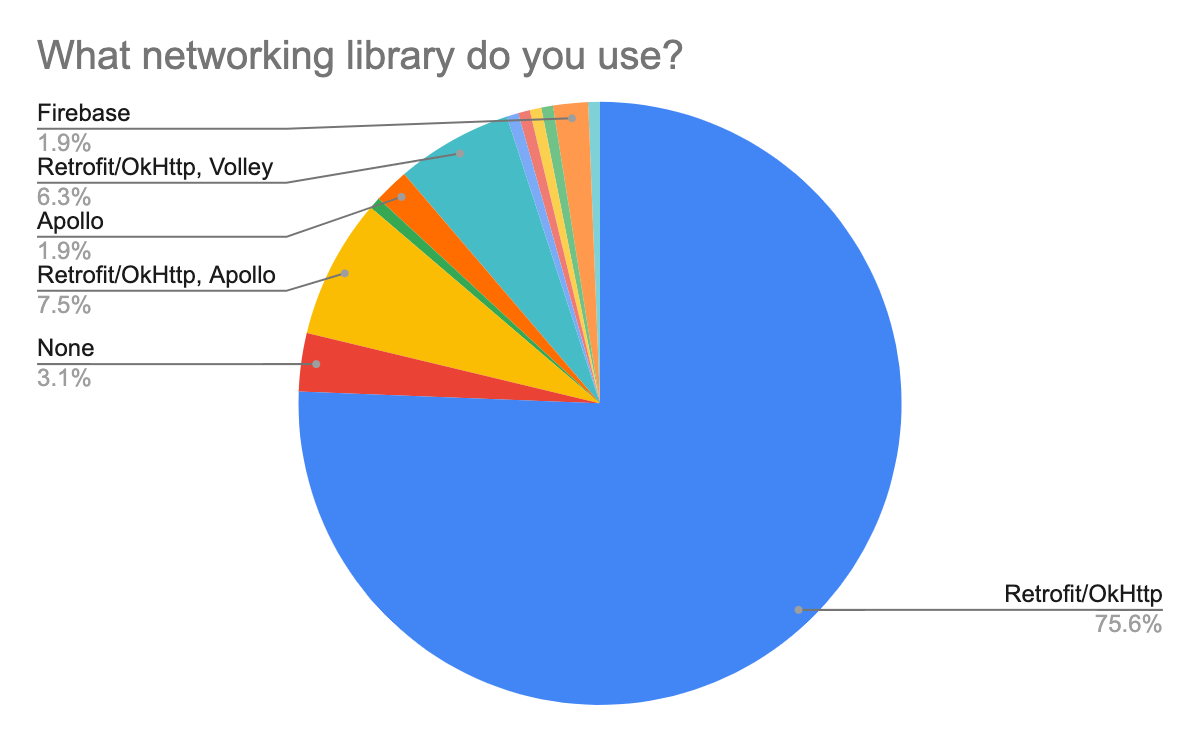
\includegraphics[scale=0.25]{figures/networking_lib.png}
    \caption{Networking library preferences results}
    \label{fig:networking_lib}
\end{figure}
\FloatBarrier

More detailed information and comments about these libraries can be found in \ref{section:4.5.2}. Mooncascade's Android team prefers Retrofit or Apollo libraries depending on the back-end system’s type to be used in the project. This preference is in line with the survey results.

The 8th question of the survey asks the question of what libraries they use to manage asynchronous processes while developing Android applications to the participants. This question was included in the survey, considering that many Android applications are based on asynchronous events and the impact of the tools used in managing these events on the application architecture and thus on maintainability. When the results are examined, it is seen that Android developers prefer the Kotlin Coroutines, RxJava and AsyncTask solutions. It is also seen that some of the participants declared that they used more than one solution. The use of more than one solution can be explained by applications that need to be maintained or preferring a solution based on the project needs. Recently, the AsyncTask solution has been deprecated by the Android team. However, it seems that some of the participants continued to use this solution. This situation can be explained by maintaining some previously coded applications using the AsyncTask and are still in use. The use of this solution is no longer recommended \footnote{\url{https://developer.android.com/reference/android/os/AsyncTask}}. Details of the results can be seen in the below in Fig.\ref{fig:async_events}.
\begin{figure}[ht!]
    \centering
    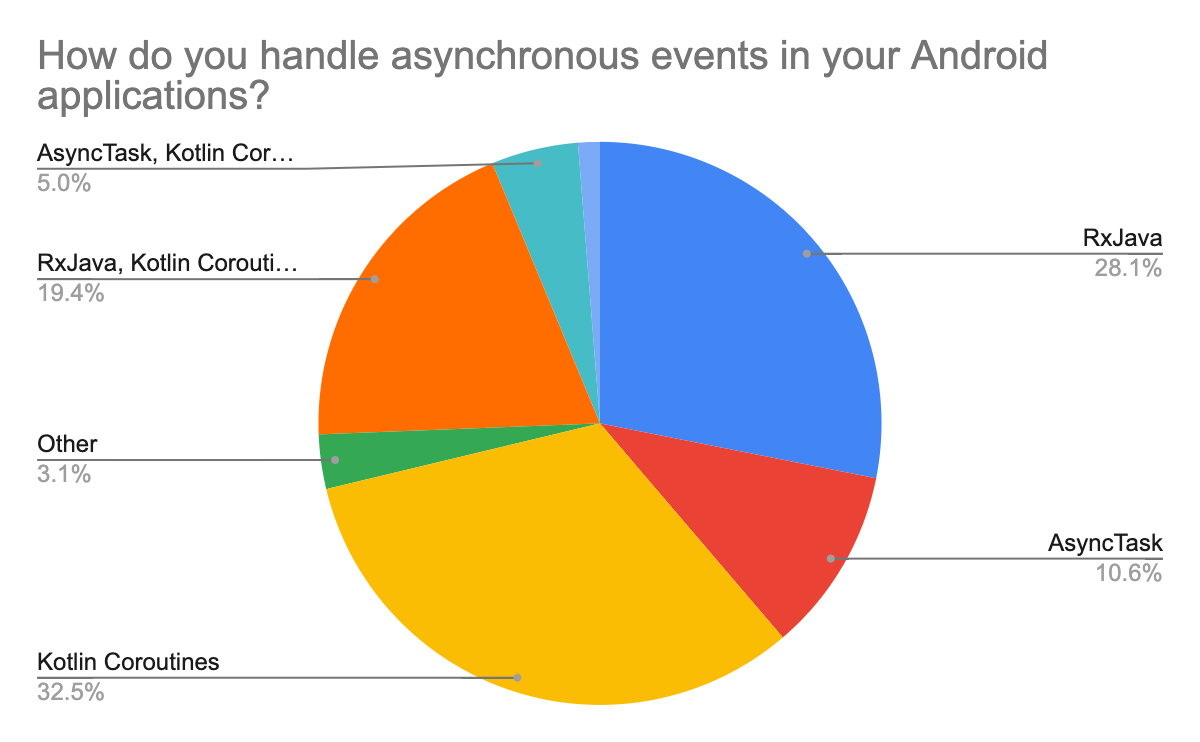
\includegraphics[scale=0.25]{figures/async_events.png}
    \caption{Threading management library preferences results}
    \label{fig:async_events}
\end{figure}
\FloatBarrier

On the other hand, we see that the Kotlin coroutines solution, which Android officially recommends \footnote{\url{https://developer.android.com/topic/libraries/architecture/coroutines}}, has the highest percentage in the survey. This solution is increasing among Android developers, as it is easier to learn and use than the RxJava library and because it requires no external dependency. Although RxJava has a steep learning curve and faces the growing popularity of the Kotlin coroutines, it is still preferred by many Android developers for the advanced features it offers. However, there has been a severe increase of applications that have recently migrated their RxJava solutions to Kotlin coroutines\cite{42}. Although the Mooncascade Android prefers RxJava for now, it has been continuing its efforts to switch to Kotlin Coroutines solution. Details on how RxJava is by used are shared in section \ref{section:4.5.3}.

The 9th question of the questionnaire asks the participants which solutions are preferred to apply dependency injection (DI) principles, which significantly impact software maintainability and software architecture when developing Android applications. As shown in Fig. \ref{fig:di_lib}, Dagger 2 is the most commonly used DI framework amongst the participant Android developers. Approximately 67.5\% of users declared that they used this solution in some way. Besides, Hilt, another DI framework developed based on Dagger 2 by Google's Android team, a relatively new technology, was able to find a place in the survey. Dagger 2 and Hilt are DI frameworks recommended by the Android team. However, it is predicted that Hilt's use will surpass Dagger 2 soon, primarily due to the ease of learning it brings and the decrease in boilerplate code  \footnote{\url{https://developer.android.com/training/dependency-injection/hilt-android}}. Apart from these solutions, the Koin DI framework also stands out among the results. It can be said that the Koin is preferred among Android developers because of its ease of learning and its ability to get integrated into Android applications with much less boilerplate code when compared to Dagger 2. Also, it is essential to mention that Koin was developed by using Kotlin programming language. Finally, it is seen that 3.1\% of the participants are not aware of the concept of DI and 17.5\% of them declared that they do not use any framework for DI. This situation is not surprising given that all of the participants, who were not aware of the concept of DI, had less than a year of experience. Because DI is an advanced software development concept, and its practical implementation is a technique that requires solid experience. It is not mandatory to use any DI framework when developing Android applications. Therefore, it can be mentioned that 17.5\% of the participants stated that they do not use any framework and apply their custom solutions. Detailed results can be seen in Fig. \ref{fig:di_lib} below.
\begin{figure}[ht!]
    \centering
    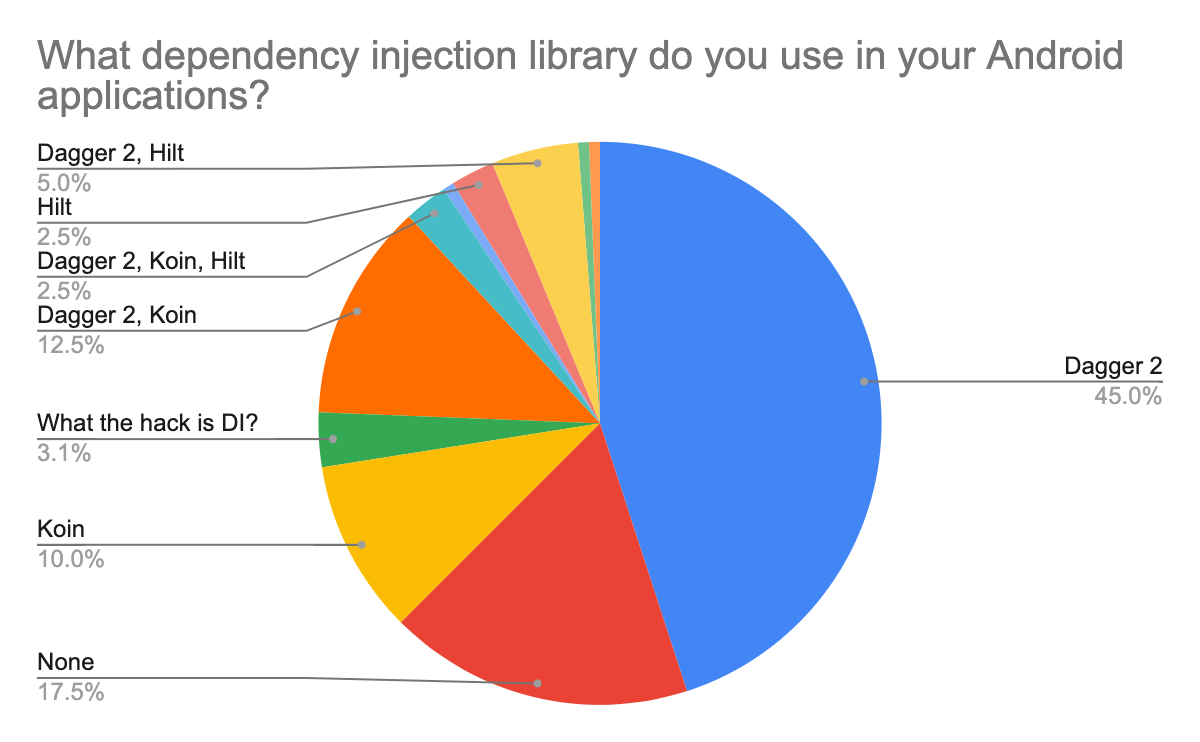
\includegraphics[scale=0.25]{figures/di_lib.png}
    \caption{DI Library preferences results}
    \label{fig:di_lib}
\end{figure}
\FloatBarrier

Mooncascade's Android team applies DI principles in their projects and makes these applications through the Dagger 2 framework. Details on how this framework is used are shared in section \ref{section:4.5.1}. The Team is also considering migrating to Hilt soon.

The final question of the survey asks respondents whether they are using the Android Architecture Components framework. When the results are examined, it is seen that more than 92\% of the participants stated that they use or can use this framework while only 7.5\% of the applicants declared that they do not use it. The high rate of usage is understandable, considering the out of box solutions it offers in solving some of the difficulties encountered while developing Android applications (which were mentioned in the first section, e.g. activity/fragment life-cycle) and the other facilities it provides for Android developers. In addition to this situation, there are groups in the Android community that are distant from this framework because it causes some other difficulties while solving the previously mentioned problems. This claim is controversial, and its details are beyond the focus of this study. However, this may be the reason why some participants do not prefer using this framework. Fig. \ref{fig:arch_components} presents the participant responses to this question in the form of a column chart.
\begin{figure}[ht!]
    \centering
    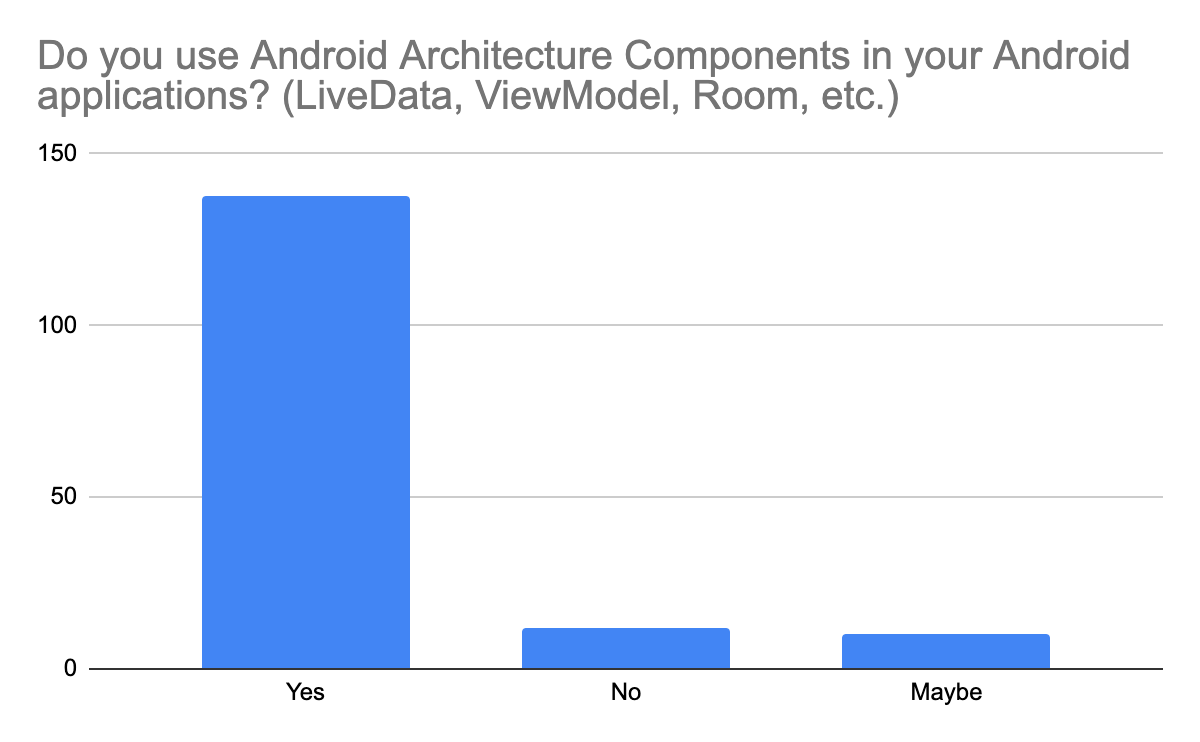
\includegraphics[scale=0.25]{figures/arch_components.png}
    \caption{Android Architecture Components usage results}
    \label{fig:arch_components}
\end{figure}
\FloatBarrier

 Mooncascade's Android team prefers to use the Android Architecture Components framework. Details on how this framework is used are shared in section \ref{section:4.5.4}.